\icode{N17-MU-SI-L3-261029-001}
\nceeID[unkown]{2017全国\Rmnum{1}}{unkown}
如图，柔软轻绳\(ON\)的一端\(O\)固定，其中间某点\(M\)拴一重物，用手拉住绳的另一端\(N\)。初始时，\(OM\)竖直且\(MN\)被拉直，\(OM\)与\(MN\)之间的夹角为\(\alpha\)（\(\alpha > \frac{\pi}{2}\)）。现将重物向右上方缓缓拉起，并保持夹角\(\alpha\)不变。在\(OM\)由竖	直被拉到水平的过程中\paren[]

\begin{tikzpicture}[font=\scriptsize]
	\draw[magenta] (0,2)node[left,black]{\(O\)}--(0,0)node[below,black]{\(M\)}--++(-30:2)node[right,black]{\(N\)};
	\draw (0,.3) arc(90:-35:.3);
	\shade[ball color=gray] (0,0) circle(.08);
	\fill (0,2)circle(.03);
	\node at(.5,.1){\(\alpha\)};
\end{tikzpicture}
\begin{choices}
	\item\(MN\)上的张力逐渐增大
	\item\(MN\)上的张力先增大后减小
	\item\(OM\)上的张力逐渐增大
	\item\(OM\)上的张力先增大后减小
\end{choices}
\begin{answer}
    AD\qquad 提示：重力与两绳上的拉力构成的外接圆如图所示
	
	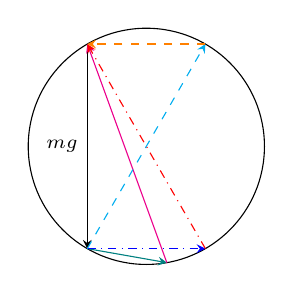
\begin{tikzpicture}[>=stealth,font=\scriptsize]
		\draw (0,0) circle(1.5);
		\draw[->] (120:1.5)--node[left]{\(mg\)}(-120:1.5);
		\draw[->,teal] (-120:1.5)--(-80:1.5);
		\draw[->,magenta] (-80:1.5)--(120:1.5);
		\draw[->,dash dot,blue] (-120:1.5)--(-60:1.5);
		\draw[->,dash dot,red] (-60:1.5)--(120:1.5);
		\draw[->,dashed,cyan] (-120:1.5)--(60:1.5);
		\draw[->,dashed,orange] (60:1.5)--(120:1.5);
	\end{tikzpicture}
\end{answer}